\documentclass{article} 
\usepackage{amsmath,amsthm}     
\usepackage{graphicx}     
\usepackage{hyperref} 
\usepackage{url}
\usepackage{amsfonts} 
\usepackage{multicol}
\usepackage{tikz}
\usepackage{smartdiagram}
\usepackage{tabularx}
\usepackage{enumitem}
\usepackage{hyperref}
\usepackage[ruled,vlined]{algorithm2e}
\usetikzlibrary{fit}
\tikzset{
	comp/.style = {
		minimum width  = 8cm,
		minimum height = 4.5cm,
		text width     = 8cm,
		inner sep      = 0pt,
		text           = green,
		align          = center,
		font           = \Huge,
		transform shape,
		thick
	},
	monitor/.style = {draw = none, xscale = 18/16, yscale = 11/9},
	display/.style = {shading = axis, left color = black!60, right color = black},
	ut/.style      = {fill = gray}
}
\tikzset{
	computer/.pic = {
		% screen (with border)
		\node(-m) [comp, pic actions, monitor]
		{\phantom{\parbox{\linewidth}{\tikzpictext}}};
		% display (without border)
		\node[comp, pic actions, display] {\tikzpictext};
		\begin{scope}[x = (-m.east), y = (-m.north)]
			% filling the lower part
			\path[pic actions, draw = none]
			([yshift=2\pgflinewidth]-0.1,-1) -- (-0.1,-1.3) -- (-1,-1.3) --
			(-1,-2.4) -- (1,-2.4) -- (1,-1.3) -- (0.1,-1.3) --
			([yshift=2\pgflinewidth]0.1,-1);
			% filling the border of the lower part
			\path[ut]
			(-1,-2.4) rectangle (1,-1.3)
			(-0.9,-1.4) -- (-0.7,-2.3) -- (0.7,-2.3) -- (0.9,-1.4) -- cycle;
			% drawing the frame of the whole computer
			\path[pic actions, fill = none]
			(-1,1) -- (-1,-1) -- (-0.1,-1) -- (-0.1,-1.3) -- (-1,-1.3) --
			(-1,-2.4) coordinate(sw)coordinate[pos=0.5] (-b west) --
			(1,-2.4) -- (1,-1.3) coordinate[pos=0.5] (-b east) --
			(0.1,-1.3) -- (0.1,-1) -- (1,-1) -- (1,1) -- cycle;
			% node around the whole computer
			\node(-c) [fit = (sw)(-m.north east), inner sep = 0pt] {};
		\end{scope}
	}
}
\DeclareMathOperator{\diag}{diag}
\DeclareMathOperator{\E}{\mathbb{E}}
\usetikzlibrary{positioning,chains,fit,shapes,calc}
\theoremstyle{theorem}
\newtheorem{theorem}{Theorem}

\theoremstyle{definition}
\newtheorem*{definition}{Definition}
\newtheorem{assumption}{Assumption}
\newtheorem*{remark}{Remark}
\newtheorem{proposition}{Proposition}

\allowdisplaybreaks
\usepackage{collectbox}
\makeatletter
\newcommand{\mybox}{%
	\collectbox{%
		\setlength{\fboxsep}{1pt}%
		\fbox{\BOXCONTENT}%
	}%
}
\@addtoreset{footnote}{page}
\makeatother

%%%%%%%%%%%%%%%%%%%%%%%%%%%%%%%%%%%%%%%%%%%%%%%%%%
\begin{document}

	\newpage
	\title{Non-convex optimization in federated learning}
	
	\author{Hoang Trung Hieu
		%\scriptsize \\    
	%Eötvös Loránd University \\               
		%hthtb22@gmail.com
	}                      
	\date{2020}
	\maketitle
	
	\noindent
	\begin{abstract}
		Federated learning (FL) is a learning paradigm seeking to address the problem of data governance and privacy by training algorithms collaboratively without exchanging the data itself. But there are some limitations: Massively distributed, non-iid dataset, the data distribution's unbalancedness. To train a neural network in general we often use the gradient decent methods to optimize the loss function. In FL, Federated Averaging(FedAvg) is used most frequently. However, it is not perfect and it performs poor-quality in some cases. My project is to analyze whether it is possible to give convergence guarantees in case the data over each devices is unbiased and evaluating of divergence between local datasets.
	\end{abstract}
	\section{Introduction}
	\subsection{Federated Learning}
	A new approach to train the model without access to the user's data is embedded machine learning. It can be described by two criteria: data never leaves the local devices and updates are communicated instead model. There are a few underlying distributed structure: peer-to-peer learning, distributed training, on-device inference and federated learning (\cite{cite1}). In this project, we consider the new paradigm in Machine Learning-Federated Learning which is a machine learning setting where multiple entities collaborate in solving a learning problem, without directly exchanging data. The Federated training process is coordinated by a central server. It works like this: your device downloads the current model, improves it by learning from data on your phone, and then summarizes the changes as a small focused update. Only this update to the model is sent to the cloud, using encrypted communication, where it is immediately averaged with other user updates to improve the shared model. All the training data remains on your device, and no individual updates are stored in the cloud.\\
	On the other hand, we face up to new challenges: \begin{itemize}
		\item \textit{Communication}.  Total communication can be calculated by the multiplication of the number of communication rounds by the number of parameters by average codeword length.It can be up to hundreds terabyte excluding the upload and download progress, but we do not mention it in this project. 
		\item \textit{Massively distributed}. The number of mobile device owners is massively bigger than average of the number of training samples on each device.
		\item \textit{Unbalanced}. Some users produce significantly more data than others.
		\item \textit{Non-IID}.	The data generated by each user are quite different.
	
\begin{center}
	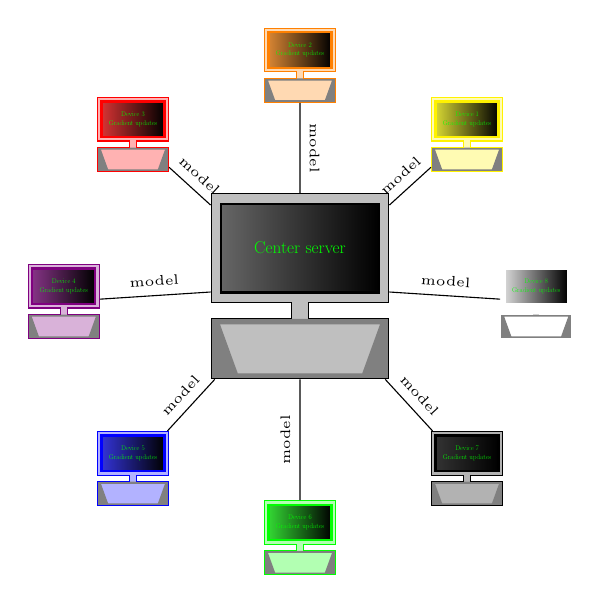
\begin{tikzpicture}
		\pic(comp0) [
		draw,
		fill = gray!50,
		scale = 0.25,
		pic text = {Center server}
		]
		{computer};
		\path(comp0-c.center) pic 
		foreach[count=\i] \farbe in {yellow, orange, red, red!50!blue, blue, green, black,white}
		(comp\i) [
		draw = \farbe,
		fill = \farbe!30,
		display/.append style = {left color=\farbe!80!black!80},
		scale = 0.1,
		pic text = {Device \i \\Gradient updates}		
		] at +(45*\i:3){computer};	
		\foreach \i in {1,2,3,4,5,6,7,8} \draw (comp\i-c) -- (comp0-c)  node [midway, above, sloped] (TextNode) {\tiny{model}};
		
	\end{tikzpicture}
\begin{center}
	\figurename[1]{. Federated Leaning structure}
\end{center}
\end{center}		
	\end{itemize}
	\subsection{Problem description}
	Let us consider the following distributed optimization model in which $N$ clients cooperatively conquer   $$\min_{w} f(w) = \min_{w} \sum_{k=1}^{N} p_k f_k(w)$$
	where $p_k$ be the weight of $k-$th device and typically it is the proportion of the local data volume in global data volume.i.e $p_k \ge 0, \quad  \sum_{i=1}^{N}p_k=1.$ The $k-$th client has $n_k$ training data which is denoted $x_{k,1} , \cdots,  x_{k,n_k}.$ The local generalization error function are defined by $$f_k(w)= \frac{1}{n_k} \sum_{j=1}^{n_k} \ell (w;x_{k,j})$$
	where $\ell$ is a user loss function of the prediction.\\
	The local generalization also can be defined by taking the expected value of training error of model parameters $w$ over local data $\xi_k \sim \mathcal{D}_k$ $$f_k(w)=\E_{\xi_k \sim \mathcal{D}_k} F(w; \xi_k)$$
	In case of the data is balanced (the volume of each device's data are equal) $$f(x)=\frac{1}{N}  \sum_{i=1}^{N} \tilde{f_k}(w) \quad \text{where} \ \ \tilde{f_k}(w) =p_kNf_k(w)$$
	\section{Algorithms}
	There are two most widely-used FL mechanisms, FedSGD and FedAvg. In general, FedSGD is barely influenced by the none
	independent and identically distributed (non-IID) data problem, but FedAvg suffers from a decline in accuracy. On the other hand, FedAvg is more efficient than FedSGD regarding time consumption and communication.
	\subsection{FedSGD}
Deep learning training mainly relies on variants of stochastic gradient descent, where gradients are computed on a random subset of the total dataset and then used to make one step of the gradient descent.

Federated stochastic gradient descent[13] is the direct transposition of this algorithm to the federated setting, but by using a random fraction C of the nodes and using all the data on this node. The gradients are averaged by the server proportionally to the number of training samples on each node, and used to make a gradient descent step.

	\subsection{FedAvg}
Federated averaging (FedAvg) is a generalization of FedSGD, which allows local nodes to perform more than one batch update on local data and exchanges the updated weights rather than the gradients. The rationale behind this generalization is that in FedSGD, if all local nodes start from the same initialization, averaging the gradients is strictly equivalent to averaging the weights themselves. Further, averaging tuned weights coming from the same initialization does not necessarily hurt the resulting averaged model's performance.	
	\begin{algorithm}[H]
		\SetAlgoLined
		\textbf{Server executes:} \\
		initialization $w_0$ \;
		\For{each round $t=1,2, \cdots $}{
			 $m \leftarrow \max(C \cdot K,1)$\\
			 $S_t \leftarrow $ (random set of $m$ client) \\
			\For{each client $k \in S_t$} {	
			$w_{t+1}^k \leftarrow \text{ClientUpdate}(k, w_t)$\;			
			}{
				$w_{t+1} \leftarrow \sum_{k=1}^{K} \dfrac{n_k}{n} w_{t+1}^k$\;
			}
		} 
	\textbf{ClientUpdate($k,w$):}\\
	$B \leftarrow \text{ (split} \ P_k	\ \text{into batches of size} \ B )$\\
	\For{each local epoch}{
	\For{batch $b \in B$}{
	$ w \leftarrow w - \eta \nabla \l(w;b)$ }}
		\caption{FederatedAveraging(FedAvg).}
	\end{algorithm}

	\section{Non-Convex optimization}
Machine learning algorithms use optimization all the time. We minimize loss, or error, or maximize some kind of score functions. Gradient descent is the "hello world" optimization algorithm covered on probably any machine learning course. It is obvious in the case of regression, or classification models, but even with tasks such as clustering we are looking for a solution that optimally fits our data (e.g. k-means minimizes the within-cluster sum of squares). So if you want to understand how the machine learning algorithms do work, learning more about optimization helps. Moreover, if you need to do things like hyperparameter tuning, then you are also directly using optimization.

One could argue that convex optimization shouldn't be that interesting for machine learning since instead of dealing with convex functions, we often face up to the composition of convex function which usually is not convex. For examples, matrix completition, principle component analysis, low-rank models and tensor decomposition, maximum likelihood estimation with hidden variables and the most important, deep neural networks.\\
In order to find convergence guarantees for non-convex function(even convex) is quite hard or unrealistic in deep learning. But there are a few assumptions that appears frequently in recent papers.
	\begin{assumption}
		\textbf{$L-$ Lipschitz gradient}: Local objective functions $f_i$ are all $L-$ smooth: $$\left\|\nabla f_i(u)-\nabla f_i(v) \right\| \leq L \left \| u-v \right\|$$
		Or it can be rewritten: $$f_i(u) \le f_i(v)+(u-v)^{T} \nabla f_i(v)+\frac{L}{2} \|u-v\|^2$$
	\end{assumption}
	\begin{assumption}
		\textbf{Bounded variance} $$\E _{\xi_k \sim D_i} \left[\| \nabla F(w, \xi_k)-\nabla f_k(w)\| ^2\right] \le\sigma ^2, \ \forall k,w $$
	\end{assumption}
\begin{assumption}
	\textbf{Bounded gradient} $$\E _{\xi_k \sim D_i} \left[\| \nabla F(w, \xi_k)\| ^2\right] \le G^2, \ \forall k,w $$
\end{assumption}
 My project is to analyze whether it is possible to give convergence guarantees in case the data over each devices is unbiased and non-iid. I believe that we need to modify the FedAvg if it guarantees the convergence in non-convex problem. In\cite{cite5}, they analyze the convergence of FedAvg on non-iid data and establish a convergence for strongly convex and smooth problems.
 
\section{Experimental results}
In most cases, the assumption of independent and identically distributed samples across local nodes does not hold for federated learning setups. Under this setting, the performances of the training process may vary significantly according to the unbalancedness of local data samples as well as the particular probability distribution of the training examples (i.e., features and labels) stored at the local nodes.\\
\textbf{Models.} The models we use in experimental part are: 2NN and CNN.
The 2NN model is a deep neural network with 2 hidden layer.\\
(fc1): Linear( input features=784, output features=200, bias=True)\\
(fc2): Linear( input features=200, output features=200, bias=True)\\
(fc3): Linear(input features=200, output features=10, bias=True)\\
The convolutional neural network is described the following:\\
(conv1): Conv2d(1, 32, kernel size=(5, 5), stride=(1, 1)) \\
(conv2): Conv2d(32, 64, kernel size=(5, 5), stride=(1, 1))\\
(fully connected 1): Linear(input features=1024, output features=512, bias=True)\\
(fully connected 2): Linear(input features=512, output features=10, bias=True)\\
\textbf{Dataset} The dataset we choose to examine is MNIST dataset. To simulate the non-IID data distribution
by setting each client to hold only digits from one certain
class and the number of clients from the same class to be
$N=100.$ To simulate the data unbalance, we let the number of
samples on each client roughly follow a power law (Figure[1.1]) .\\
\begin{center}
		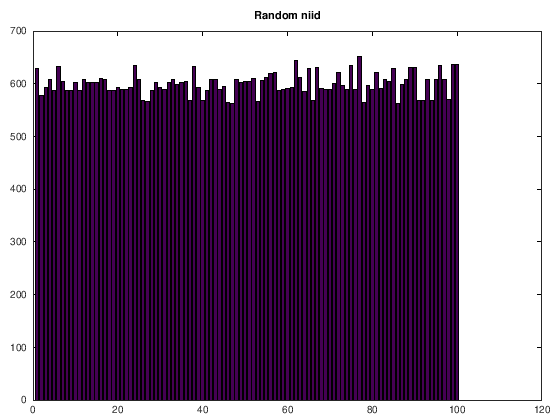
\includegraphics[scale=0.2]{random_niid.png}
		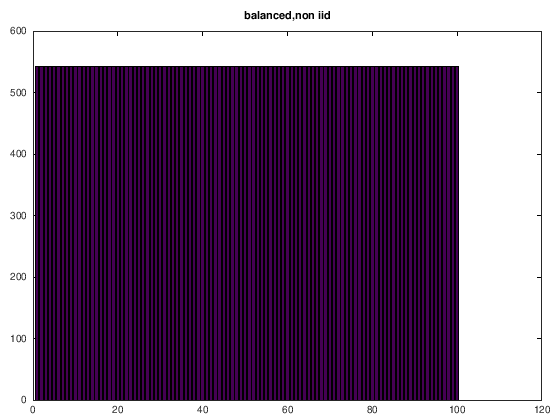
\includegraphics[scale=0.2]{equal.png}
\end{center}
		\figurename[1.1]{. Unbalanced (left) and balanced (right) data distribution}\\
We also take the synthetic data into account. We generated synthetic data with parameters $\alpha , \beta$ where $\alpha$ can be comprehended as the differences between local datas and each other and $\beta$ is how much the local data at each device differs from that of other devices. Namely, The output of each sample can be represented as $y=\text{softmax}(W_kx+b_k)$ with $x,b_k \in \mathbb{R}^{60}$ and $W_k \in \mathbb{R}^{10 \times 60}$. We model each entry of $W_k$ and $b_k$ as $\mathcal{N} (\mu_k,1)$ with $\mu_k \sim \mathcal{N}(0, \alpha)$ and $(x)_{kj} \sim  \mathcal{N}(v_k, 1/j^{1.2})$ with $v_k \sim \mathcal{N}(\mathcal{N}(0, \beta), 1)$.\\
			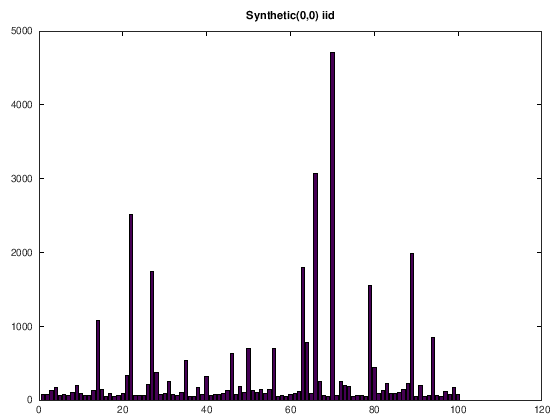
\includegraphics[scale=0.15]{sy00iid.png}
			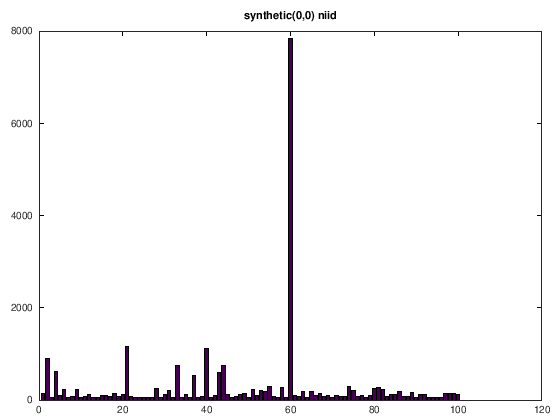
\includegraphics[scale=0.15]{sy00niid.png}
			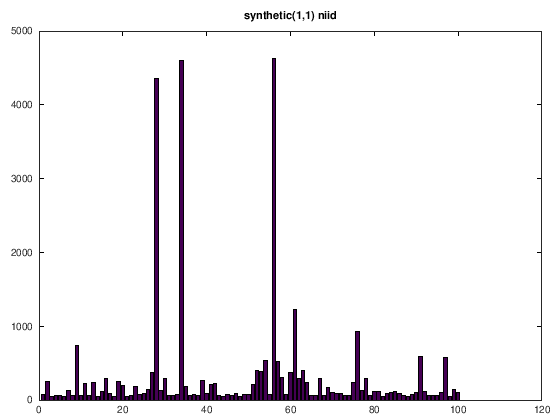
\includegraphics[scale=0.15]{sy11.png}
			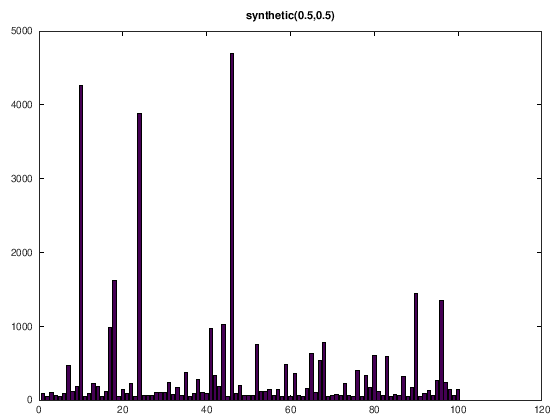
\includegraphics[scale=0.15]{sy0.50.5.png}
						\figurename[1.2]{. Synthetic data with $(\alpha, \beta) =(0,0)$-iid ,$(\alpha, \beta) =(0,0)$-niid,$(\alpha, \beta) =(1,1)$-niid,$(\alpha, \beta) =(0.5,0.5)$-niid (from left to right)  }\\					
\textbf{Notation of parameters.}\\
Number of federated learning rounds: T\\
Total number of nodes used in the process: K\\
Fraction of nodes used at each iteration for each node: C\\
Local batch size used at each learning iteration: B\\
Number of iterations for local training before pooling: $N$\\
Local learning rate: $\eta $\\
Regularzation parameter: $\lambda$ \\
\textbf{Set up}. For all experiments the initial weight is $w_0=0$ and each round the selected device run $E$ steps of SGD in parallel. 					\\
\textbf{Impact of parameters}
To evaluate the impact of number of devices each update, we examine on Synthetic(0,0) iid (right) and non-iid (left) dataset, $ B=64, T=50,lr=0.01,E=5$, model is 2NN. The value of $C$ in the set $\{5/100,10/100,20/100,50/100\}$. The horizontal axis is the train loss.
\begin{center}
		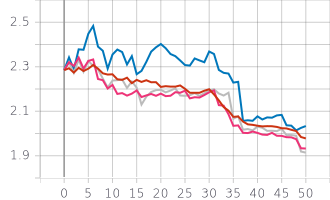
\includegraphics[scale=0.5]{Cniid.png}
			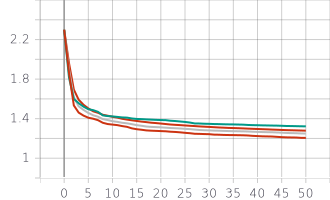
\includegraphics[scale=0.5]{Ciid.png} \\
	\figurename[3.1]{. Impact of C}
\end{center}
To evaluate the impact of number of epoch, we examine on MNIST unbalanced non-iid dataset, $C=5/100, B=64, T=50,lr=0.01$, model is CNN. The value of $E$ in the set $\{2,5,10,20\}$. The horizontal axis is the train accuracy.
\begin{center}
	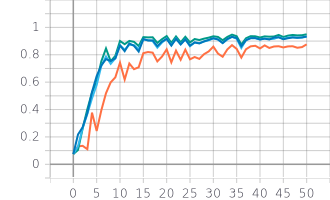
\includegraphics[scale=0.65]{E.png}\\
	\figurename[3.2]{. Impact of E}
\end{center}
To evaluate the impact of batch size, we examine on MNIST balanced non-iid dataset, $C=10/100, T=50,lr=0.01$, model is 2NN. The value of $B$ in the set $\{16,32,64,128\}$. The horizontal axis is the test accuracy.
\begin{center}
	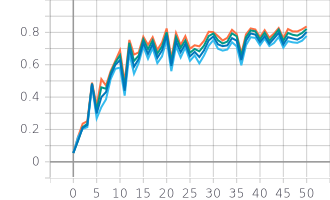
\includegraphics[scale=0.65]{B.png}\\
	\figurename[3.3]{. Impact of B}
\end{center}
\textbf{Impact of balancedness.} To evaluate the impact unbalancedness, we examine on Synthetic dataset with different parameters $\alpha , \beta$, namely Synthetic data with $(\alpha, \beta) =(0,0)$-iid ,$(\alpha, \beta) =(0,0)$-niid,$(\alpha, \beta) =(1,1)$-niid,$(\alpha, \beta) =(0.5,0.5)$-niid $C=10/100, B=64, T=50,lr=0.01, E=5$, model is CNN. The horizontal axis is the test loss.
\begin{center}
		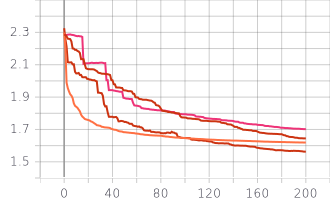
\includegraphics[scale=0.65]{syn.png}\\
\figurename[3.4]{. Impact of unbalancedness}
\end{center}
	\begin{thebibliography}{5}
	\bibitem{cite0}
	V. Felbab, P. Kiss, and T. Horváth, (2019), \textit{Optimization in Federated Learning},ITAT 2019
	
	
	\bibitem{cite1}
	F. Sattler, S. Wiedemann, K. Müller, W. Samek,  (2019), \textit{Robust and communication-efficient federated learning from non-iid data},IEEE transactions on neural networks and learning systems,
	\bibitem{cite2}
	H. Brendan McMahan, Eider Moore, Daniel Ramage, (2017) , \textit{Communication-Efficient Learning of Deep Networks
		from Decentralized Data}, \href{https://arxiv.org/abs/1602.05629}{https://arxiv.org/abs/1602.05629}	
	\bibitem{cite31}
	\textit{On the Convergence of FedAvg on Non-IID Data
		repository}, \href{ https://github.com/lx10077/fedavgpy }{https://github.com/lx10077/fedavgpy}	
	\bibitem{cite5}
	X. Li, K. Huang, W. Yang, S. Wang, Z. Zhang, (2019),  \textit{On the Convergence of FedAvg on Non-IID Data}, \href{https://arxiv.org/abs/1907.02189}{https://arxiv.org/abs/1907.02189}
	\bibitem{cite6}
	J. Konečný, H. B. McMahan, D. Ramage, P. Richtárik, (2016),  \textit{	Federated Optimization Distributed Machine Learning for On-Device Intelligence} \href{https://arxiv.org/abs/1610.02527}{https://arxiv.org/abs/1610.02527}
	\bibitem{cite7}
	A. K. Sahu, T. Li, M. Sanjabi, M. Zaheer, A. Talwalkar, and V. Smith, (2018), 
	\textit{Federated optimization for heterogeneous networks}, \href{https://arxiv.org/abs/1812.06127}{https://arxiv.org/abs/1812.06127}
\end{thebibliography}

\end{document}